  \begin{figure}[h!]
    \centering
    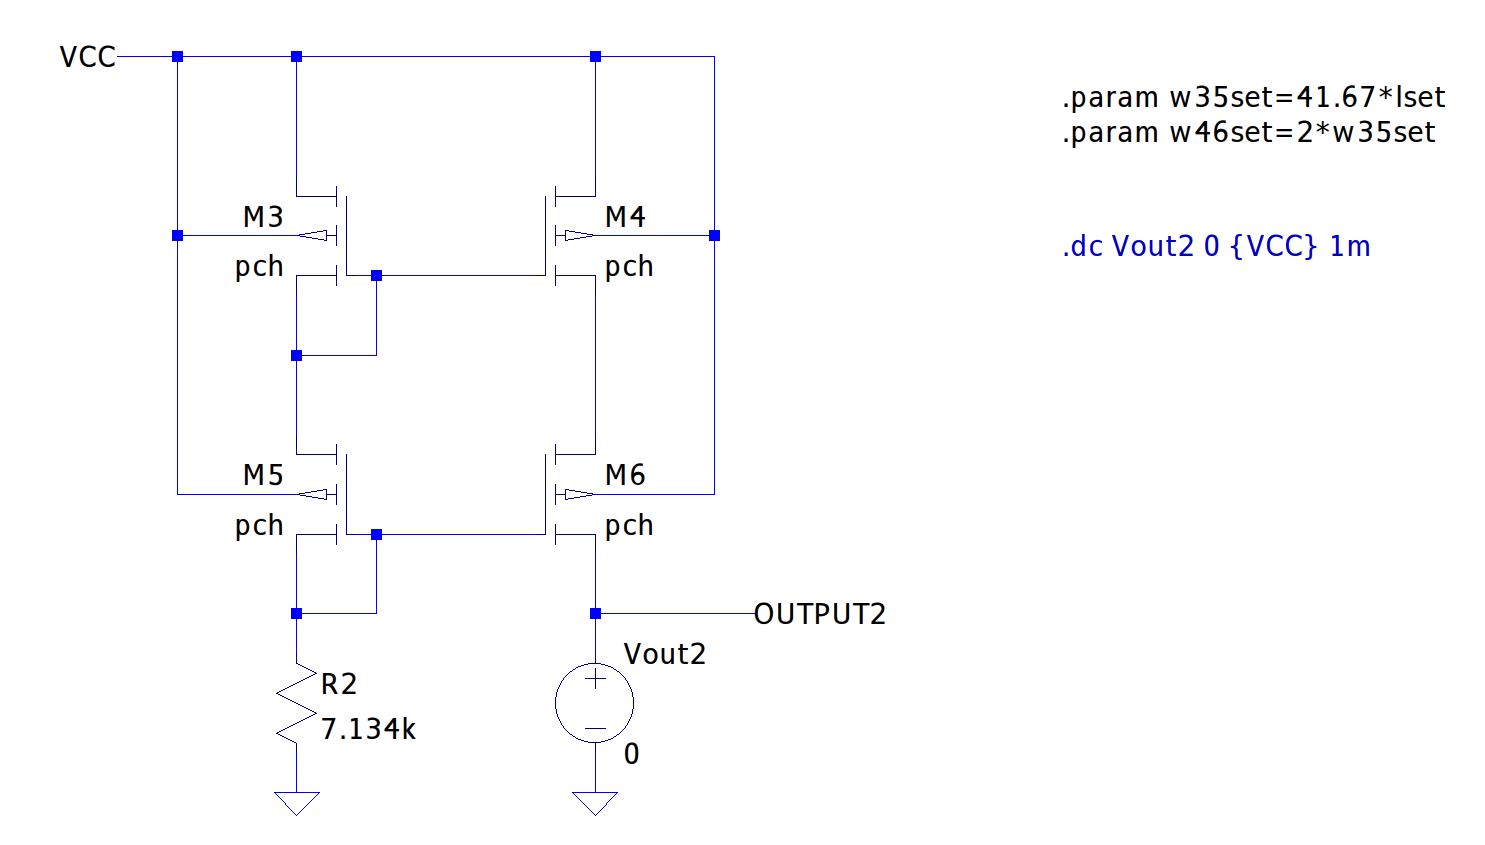
\includegraphics[scale=0.5]{spice2.png}
    \caption{Proudová reference, analýza OP.}
    \label{fig:spice0-png}
  \end{figure}

  \begin{figure}[h!]
    \centering
    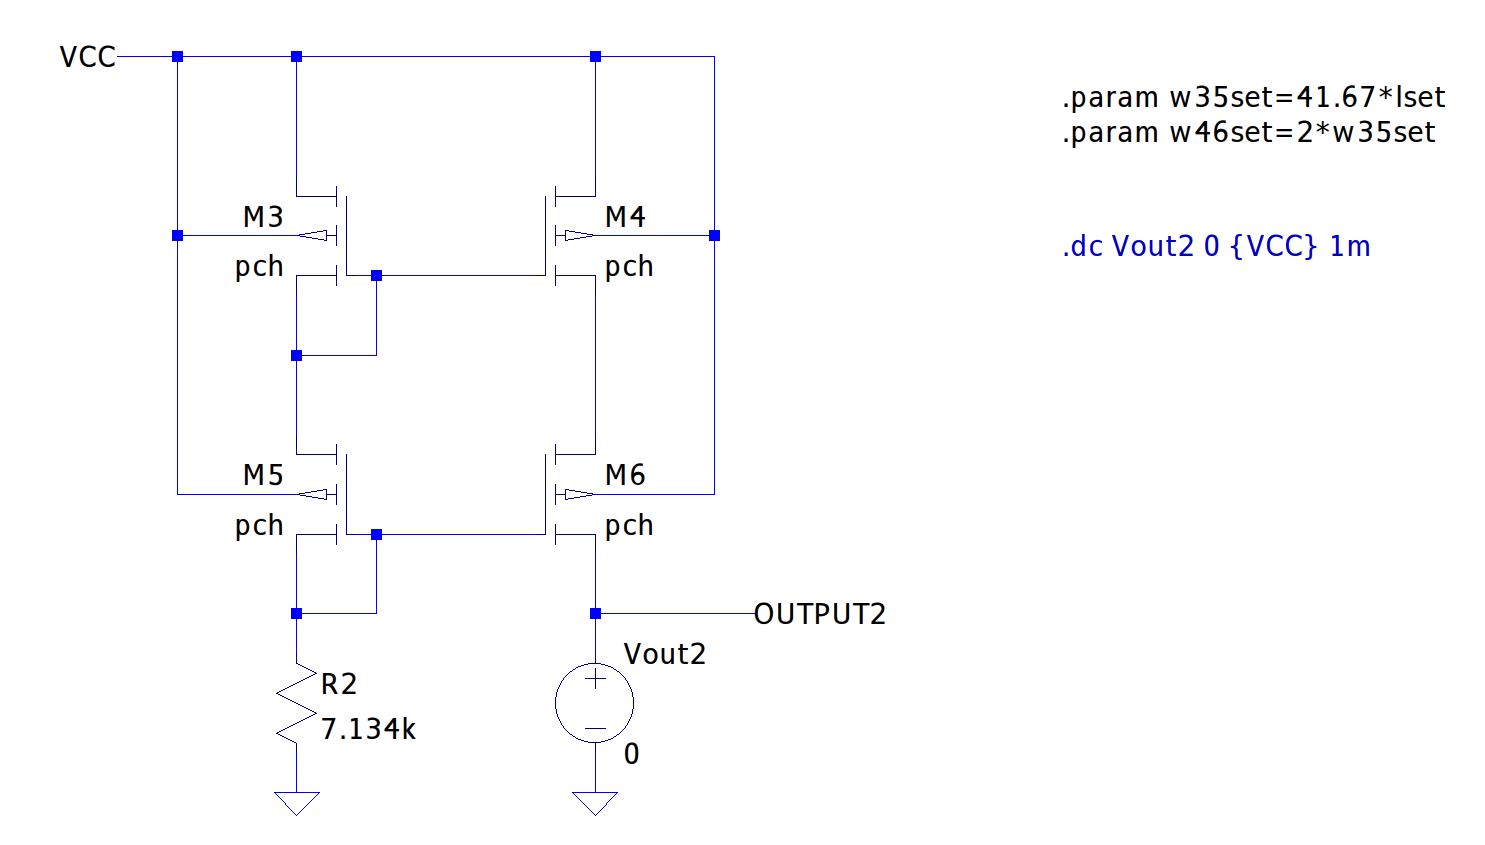
\includegraphics[scale=0.5]{spice2.png}
    \caption{Proudová reference, analýza OP -- C2 vnutí prac. bod.}
    \label{fig:spice0-png}
  \end{figure}

  \begin{figure}[h!]
    \centering
    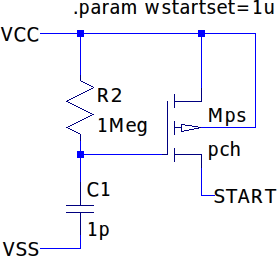
\includegraphics[scale=0.5]{spice1.png}
    \caption{Startovací obvod.}
    \label{fig:spice0-png}
  \end{figure}


\clearpage
\subsubsection{Ruční návrh}
Nejprve vypočítám rozměry pro tranzistor \(M_{N1} \):
\[
    \frac{W_{N1} }{L}=\frac{2\cdot I_{D}}{KP_{N}\cdot (U_{GS} -U_{TH})^2 } 
\]
\[
    \frac{W_{N1} }{L}=\frac{2\cdot \num{20e-6}}{\num{220e-6}\cdot (\num{0.2})^2 } 
\]

\[
    \frac{W_{N1} }{L}\doteq \num[round-mode=places,round-precision=2]{4.545454545454545} 
\]
Délku \(L\) zvolíme opět \qty{2}{\micro\meter}, tedy \(W_{N1}= \qty{9.09}{\micro\meter}\). Pro tranzistor \(M_{N2} \) zvolíme stejné rozměry.

Pro tranzistory \(M_{P1} \) a \(M_{P2} \) vypočteme rozměry obdobným způsobem:

\[
    \frac{W_{P12} }{L}=\frac{2\cdot I_{D}}{KP_{P}\cdot (U_{GS} -U_{TH})^2 } 
\]
\[
    \frac{W_{P12} }{L}=\frac{2\cdot \num{20e-6}}{\num{60e-6}\cdot (\num{0.2})^2 } 
\]

\[
    \frac{W_{P12} }{L}\doteq \num[round-mode=places,round-precision=2]{16.666666666666664}
\]

Pro stejnou délku \(L\) pak vychází \(W_{P12}=\qty{33.33}{\micro\meter} \).

Dále je potřeba stanovit hodnotu odporu \(R_{1} \), úbytek napětí na něm odpovídá napětí napětí \(U_{GS} \) pro tranzistor \(M_{N1} \):
\begin{align*}
    R_{1} =& \frac{U_{R1}}{I_{R1}} \\
          =& \frac{U_{GS,M1}}{I_{M,N2}} \\
          =& \frac{U_{TH0,N1}+U_{OV,N1} }{I_{M,N2}} \\
          =& \frac{\num{360e-3}+\num{0.2} }{\num{20e-6}} \\
          =& \qty{28}{\kilo\ohm}
\end{align*}

Pro výstupní větev je požadován jiný proud, upravíme tedy rozměry tranzistoru \(M_{P3} \):
\begin{align*}
    W_{P3} =& \frac{3}{2}\cdot W_{P2} \\
           =& \frac{3}{2}\cdot \num{16.67} \\
           =& \qty{25}{\micro\meter}
\end{align*}

Výstupní odpor zapojení je dán tranzistorem \(M_{P3} \):
\[
    r_{OUT} = \frac{1}{\lambda I_{MP3} }=\frac{1}{\num{0.08}\cdot \num{30e-6}}=\qty{416.67}{\kilo\ohm}
\]

\subsubsection{Simulace}

\begin{figure}[h!]
    \centering
    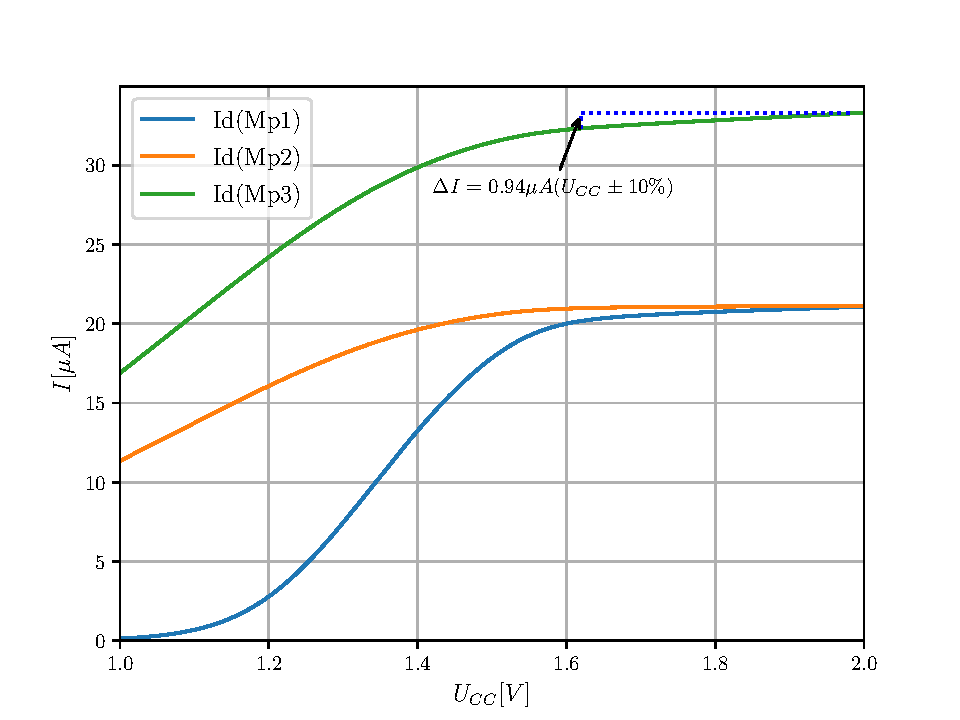
\includegraphics[width=0.8\textwidth]{img/3-1-4.pdf}
    \caption{Závislost proudů v obvodu na změně napájecího napětí.}
    \label{fig:img/3-1-4.pdf}
\end{figure}


\begin{figure}[h!]
    \centering
    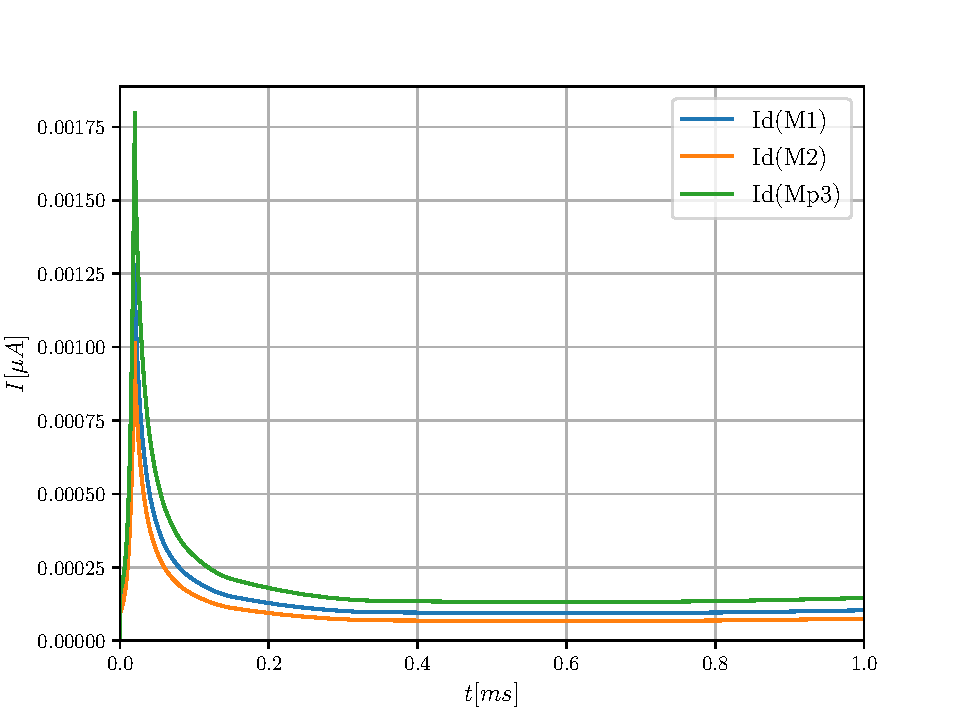
\includegraphics[width=0.8\textwidth]{img/3-1-5.pdf}
    \caption{Časová analýza zapojení bez startovacího obvodu (sw1=closed).}
    \label{fig:img/3-1-5.pdf}
\end{figure}

\begin{figure}[h!]
    \centering
    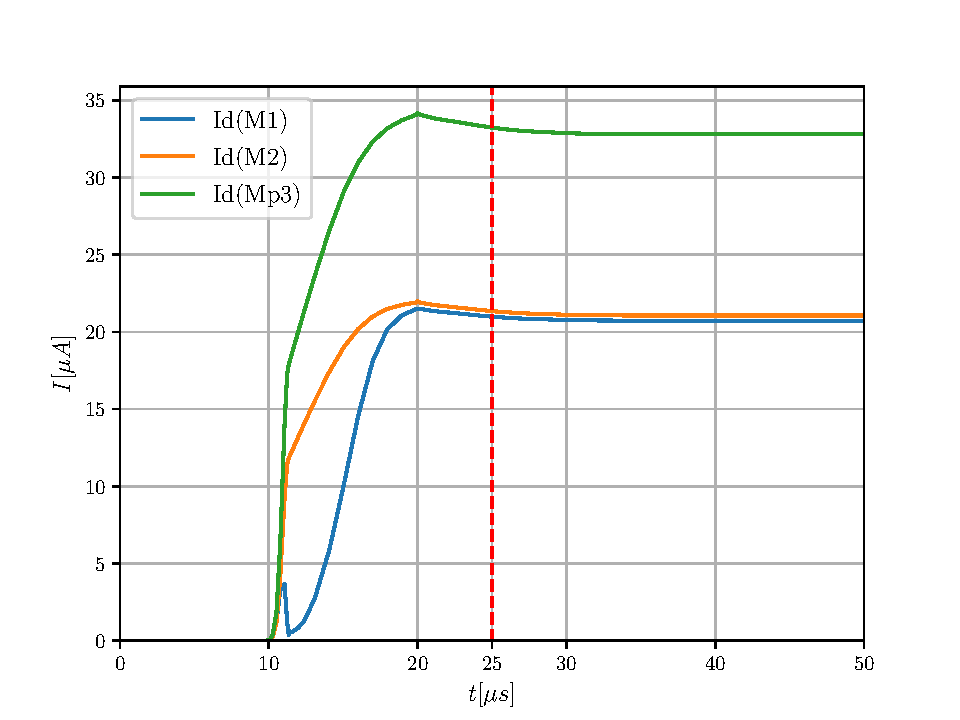
\includegraphics[width=0.8\textwidth]{img/3-1-6.pdf}
    \caption{Časová analýza zapojení se startovacím obvodem (sw1=open).}
    \label{fig:img/3-1-6.pdf}
\end{figure}